
%
%  $Description: Author guidelines and sample document in LaTeX 2.09$ 
%
%  $Author: ienne $
%  $Date: 1995/09/15 15:20:59 $
%  $Revision: 1.4 $
%

\documentclass[times, 10pt,twocolumn]{article} 
\usepackage{latex8}
\usepackage{times}

\usepackage{amsfonts}
\usepackage{amsmath}
\usepackage{boxedminipage}
%\usepackage{epsf}
\usepackage[latin1]{inputenc}
%\usepackage{babel}
\usepackage{graphicx}
\usepackage{setspace}

%\documentstyle[times,art10,twocolumn,latex8]{article}

%------------------------------------------------------------------------- 
% take the % away on next line to produce the final camera-ready version 
\pagestyle{empty}

%------------------------------------------------------------------------- 
\begin{document}

\title{Using MiBench on Cache Compression tests}

\author{Anderson Briglia\\
Universidade Federal do Amazonas\\ Departamento de Ci�ncia da Computa��o \\ Av. 
General Rodrigo Otavio, Manaus-Amazonas, Brazil\\ anderson.briglia@gmail.com\\
% For a paper whose authors are all at the same institution, 
% omit the following lines up until the closing ``}''.
% Additional authors and addresses can be added with ``\and'', 
% just like the second author.
\and
Edward David Moreno\\
UEA\\
First line of institution2 address\\ Second line of institution2 address\\ 
edwdavid@gmail.com\\
}

\maketitle
\thispagestyle{empty}

\begin{abstract}
Cache memory compression was originally developed for desktop and server platforms, but has also attracted interest on embeded systems where memory is generally a scarce resource, and hardware changes bring more costs and energy consumption. The project evaluated in this paper acts in RAM memory of embedded devices, creating a virtual compressed area for memory swapping. The tests included in MiBench were used to test this new memory hierarchy. We will describe the Compressed Cache design and tests methodology used to test the memory consumption behavior.
\end{abstract}



%------------------------------------------------------------------------- 
\Section{Introduction}

Most of embedded systems has as common characteristic: your usage for single specific tasks. But embedded systems for general purpose are pretty common as well \cite{mor00}. Linux is an Operational System which can be used in embedded devices. Embedded devices, such as PDA's (Personal Data Assistance), netbooks and Internet tablets, can use Linux as Operational System, allowing users to have access to multimedia content and other tasks which demands a higher processing capacity and memory storage.

Regarding processor power, there is no much to do instead of change the processor. But, for memory capacity, there are some solutions that do not depend on hardware changes. Compressed caching is the introduction of a new level into the virtual memory hierarchy.\cite{briglia07, castro03}. RAM (Random Access Memory), is used to store normal memory pages and compressed memory pages. Creating a reserved area called ramzswap, Compressed Cache uses this area for memory swapping. As used by several Operational Systems, swap areas intends to increase the virtual memory storage.

As presented in \cite{briglia07}, not only input and output rates could be improved when Compcache is used, but also the system behavior. Especially in memory-critical cases leading, Compcache can be used to ameliorate the Out-of-memory conditions. Tests used in \cite{briglia07} did not use MiBench \cite{GRE01} to evaluate the memory consumption behavior. Since MiBench is largely used in embedded systems evaluations, this paper presents Compcache usage against MiBench benchmarks.

%------------------------------------------------------------------------- 
\Section{Compressed Caching}

\subsection{Linux Virtual Memory Overview}

Physical pages are the basic unit of memory management \cite{love05kerneldevel} and the MMU is the hardware that translates virtual pages addresses into physical pages address and vice-versa. This compressed caching implementation, CCache \cite{ccache06}, adds some new flags to help with compressed pages identification and uses the same lists used by the PFRA (Page Frame Reclaiming Algorithm). When the system is under a low memory condition, it evicts pages from memory. It uses Least Recently Used (LRU) criteria to determine order in which to evict pages. It maintains two LRU lists---active and inactive LRU lists. These lists may contain both page-cache (file-backed) and swap-cache (anonymous) pages. When under memory pressure, pages in inactive list are freed as:

\begin{itemize}
\item Swap-cache pages are written out to swap disks using swapper\_space writepage() (swap\_writepage()).

\item Dirty page-cache pages are flushed to filesystem disks using filesystem specific writepage().

\item Clean page-cache pages are simply freed.
\end{itemize}

\subsubsection{About Swap Cache}

This is the cache for anonymous pages. All swap cache pages are part of a single swapper\_space. A single radix tree maintains all pages in the swap cache. swp\_entry\_t is used as a key to locate the corresponding pages in memory. This value identifies the location in swap device reserved for this page.

\subsubsection{About Page Cache}
This is the cache for file-system pages. Like swap cache, this also uses radix-tree to keep track of file pages. Here, the offset in file is used as the search key. Each open file has a separate radix-tree. For pages present in memory, the corresponding radix-node points to struct page for the memory page containing file data at that offset.

\SubSection{Compressed Cache Overview}
Compressed Cache (Compcache), is a technique which adds a new level in Linux memory hierarchy \cite{castro03, douglis93, kaplan99compressed}. Compcache is used to improve the memory pages access time in Linux kernel, storing more pages in RAM memory instead of slow block devices (used in regular swap\footnote{Swap area is a reserved portion from the filesystem which intends to increase the available virtual memory amount, improving the free memory for user applications.} areas) and avoiding that more pages were discarded. It is known that swap areas are slower than main memory, because block devices (usually hard disks), have higher access time rates for Input/Output operations. For embedded systems the problem is worst since swap area is generally not present in such systems.

Using the same compression algorithm present in JFFS2 filesystems (LZO \cite{obe05lzo, ZivLem77}), swap selected memory pages are compressed and sent to the virtual swap area, called ramzswap. This virtual swap acts like a block device with a swap partition and from Linux kernel point of view, there is no difference from a regular swap partition and ramzswap swap partition. Virtual compressed swap is self-contained and the compression and decompression is done when a page is inserted or retrieved from Compcache. See Figure \ref{fig:compcache}.

\begin{figure}[htb]
 \centering
 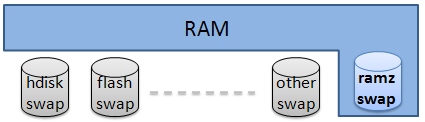
\includegraphics[scale=0.5]{figs/compcache.png}
 % compcache.png: 425x122 pixel, 72dpi, 14.99x4.30 cm, bb=0 0 425 122
 \caption{Swap with virtual block device -- ramzswap.}
 \label{fig:compcache}
\end{figure}

\subsubsection{Implementation Design}

A virtual block device is configured to have a swap partition and is added to system swaps table. Doing this, the PFRA is used to select the swappable pages and sent them to virtual compressed area (ramzswap).

To avoid fragmentation and improve efficiency, a new memory allocator was developed for Compcache. xvMalloc \cite{ccache09} is based on TLSF (Two Level Segregate Fit) allocator \cite{Masmano04}, which was developed for real-time systems.

General purpose memory allocator, generally are designed to handle allocations bigger than 4 kilobytes, which is the default size for memory pages, on Linux. This new allocator, xvMalloc, is designed to work with very tiny memory allocations, for example 32 bytes, or $3/4$ of default page size. Due to this page size characterist, fragmentation must be avoided since performance is an important issue.

Inherited from TLSF \cite{Masmano04}, xvMalloc \cite{ccache09} has some useful features that are used in Compcache:

\begin{itemize}
\item O(1) Alloc/Free: Except for cases where xvMalloc has to go to system page allocator to get additional memory.
\item Very low fragmentation: In all tests, xvMalloc memory usage is within 12$\%$ of ``Ideal'' allocator.
\end{itemize}

But, xvMalloc has added new features \cite{ccache09}, as follow:

\begin{itemize}
 \item Allocation size is always in range [MIN, MAX] and this is range is small. For Compcache this range is, for example $[32, 3/4 * PAGE_SIZE]$. This avoid fragmentation.
 \item Memory being managed is not backed by any VA. Allocator records $<$pageNum, offset$>$ for each object.
 \item Per object overhead is 4 bytes. In TLSF, this value is 16 bytes.
 \item xvMalloc stores \textbf{exact} object size in object header. This saves additional 2 bytes per object since it is not necessary to store data section beginning.
\end{itemize}

From kernel point-of-view, ramzswap is a normal swap area and must provide a small access time for compressed pages. Low fragmentation results in less time when a compressed page is required by the memory management system. Another important feature implemented by xvMalloc is the size of meta-data for each object. With 4 bytes for each object (or compressed page), more space can be used to store compressed pages itself. The Compcache version presented in \cite{briglia07}, meta-data size is an issue because important bytes were spent to address the compressed pages.

%------------------------------------------------------------------------- 
\subsubsection{Compressed Pages Storage}
TODO

\subsubsection{Insertion and Removal Pages Operations}
TODO

\subsection{Using MiBench to test Compressed Cache}
TODO

\subsubsection{Test results}
TODO

\SubSection{Conclusions}
TODO

% All manuscripts must be in English.
% 
% %------------------------------------------------------------------------- 
% \SubSection{Printing your paper}
% 
% Print your properly formatted text on high-quality, $8.5 \times 11$-inch 
% white printer paper. A4 paper is also acceptable, but please leave the 
% extra 0.5 inch (1.27 cm) at the BOTTOM of the page.
% 
% %------------------------------------------------------------------------- 
% \SubSection{Margins and page numbering}
% 
% All printed material, including text, illustrations, and charts, must be 
% kept within a print area 6-7/8 inches (17.5 cm) wide by 8-7/8 inches 
% (22.54 cm) high. Do not write or print anything outside the print area. 
% Number your pages lightly, in pencil, on the upper right-hand corners of 
% the BACKS of the pages (for example, 1/10, 2/10, or 1 of 10, 2 of 10, and 
% so forth). Please do not write on the fronts of the pages, nor on the 
% lower halves of the backs of the pages.
% 
% 
% %------------------------------------------------------------------------ 
% \SubSection{Formatting your paper}
% 
% All text must be in a two-column format. The total allowable width of 
% the text area is 6-7/8 inches (17.5 cm) wide by 8-7/8 inches (22.54 cm) 
% high. Columns are to be 3-1/4 inches (8.25 cm) wide, with a 5/16 inch 
% (0.8 cm) space between them. The main title (on the first page) should 
% begin 1.0 inch (2.54 cm) from the top edge of the page. The second and 
% following pages should begin 1.0 inch (2.54 cm) from the top edge. On 
% all pages, the bottom margin should be 1-1/8 inches (2.86 cm) from the 
% bottom edge of the page for $8.5 \times 11$-inch paper; for A4 paper, 
% approximately 1-5/8 inches (4.13 cm) from the bottom edge of the page.
% 
% %------------------------------------------------------------------------- 
% \SubSection{Type-style and fonts}
% 
% Wherever Times is specified, Times Roman may also be used. If neither is 
% available on your word processor, please use the font closest in 
% appearance to Times that you have access to.
% 
% MAIN TITLE. Center the title 1-3/8 inches (3.49 cm) from the top edge of 
% the first page. The title should be in Times 14-point, boldface type. 
% Capitalize the first letter of nouns, pronouns, verbs, adjectives, and 
% adverbs; do not capitalize articles, coordinate conjunctions, or 
% prepositions (unless the title begins with such a word). Leave two blank 
% lines after the title.
% 
% AUTHOR NAME(s) and AFFILIATION(s) are to be centered beneath the title 
% and printed in Times 12-point, non-boldface type. This information is to 
% be followed by two blank lines.
% 
% The ABSTRACT and MAIN TEXT are to be in a two-column format. 
% 
% MAIN TEXT. Type main text in 10-point Times, single-spaced. Do NOT use 
% double-spacing. All paragraphs should be indented 1 pica (approx. 1/6 
% inch or 0.422 cm). Make sure your text is fully justified---that is, 
% flush left and flush right. Please do not place any additional blank 
% lines between paragraphs. Figure and table captions should be 10-point 
% Helvetica boldface type as in
% \begin{figure}[h]
%    \caption{Example of caption.}
% \end{figure}
% 
% \noindent Long captions should be set as in 
% \begin{figure}[h] 
%    \caption{Example of long caption requiring more than one line. It is 
%      not typed centered but aligned on both sides and indented with an 
%      additional margin on both sides of 1~pica.}
% \end{figure}
% 
% \noindent Callouts should be 9-point Helvetica, non-boldface type. 
% Initially capitalize only the first word of section titles and first-, 
% second-, and third-order headings.
% 
% FIRST-ORDER HEADINGS. (For example, {\large \bf 1. Introduction}) 
% should be Times 12-point boldface, initially capitalized, flush left, 
% with one blank line before, and one blank line after.
% 
% SECOND-ORDER HEADINGS. (For example, {\elvbf 1.1. Database elements}) 
% should be Times 11-point boldface, initially capitalized, flush left, 
% with one blank line before, and one after. If you require a third-order 
% heading (we discourage it), use 10-point Times, boldface, initially 
% capitalized, flush left, preceded by one blank line, followed by a period 
% and your text on the same line.
% 
% %------------------------------------------------------------------------- 
% \SubSection{Footnotes}
% 
% Please use footnotes sparingly%
% \footnote
%    {%
%      Or, better still, try to avoid footnotes altogether.  To help your 
%      readers, avoid using footnotes altogether and include necessary 
%      peripheral observations in the text (within parentheses, if you 
%      prefer, as in this sentence).
%    }
% and place them at the bottom of the column on the page on which they are 
% referenced. Use Times 8-point type, single-spaced.
% 
% 
% %------------------------------------------------------------------------- 
% \SubSection{References}
% 
% List and number all bibliographical references in 9-point Times, 
% single-spaced, at the end of your paper. When referenced in the text, 
% enclose the citation number in square brackets, for example~\cite{ex1}. 
% Where appropriate, include the name(s) of editors of referenced books.
% 
% %------------------------------------------------------------------------- 
% \SubSection{Illustrations, graphs, and photographs}
% 
% All graphics should be centered. Your artwork must be in place in the 
% article (preferably printed as part of the text rather than pasted up). 
% If you are using photographs and are able to have halftones made at a 
% print shop, use a 100- or 110-line screen. If you must use plain photos, 
% they must be pasted onto your manuscript. Use rubber cement to affix the 
% images in place. Black and white, clear, glossy-finish photos are 
% preferable to color. Supply the best quality photographs and 
% illustrations possible. Penciled lines and very fine lines do not 
% reproduce well. Remember, the quality of the book cannot be better than 
% the originals provided. Do NOT use tape on your pages!
% 
% %------------------------------------------------------------------------- 
% \SubSection{Color}
% 
% The use of color on interior pages (that is, pages other
% than the cover) is prohibitively expensive. We publish interior pages in 
% color only when it is specifically requested and budgeted for by the 
% conference organizers. DO NOT SUBMIT COLOR IMAGES IN YOUR 
% PAPERS UNLESS SPECIFICALLY INSTRUCTED TO DO SO.
% 
% %------------------------------------------------------------------------- 
% \SubSection{Symbols}
% 
% If your word processor or typewriter cannot produce Greek letters, 
% mathematical symbols, or other graphical elements, please use 
% pressure-sensitive (self-adhesive) rub-on symbols or letters (available 
% in most stationery stores, art stores, or graphics shops).
% 
% %------------------------------------------------------------------------ 
% \SubSection{Copyright forms}
% 
% You must include your signed IEEE copyright release form when you submit 
% your finished paper. We MUST have this form before your paper can be 
% published in the proceedings.
% 
% %------------------------------------------------------------------------- 
% \SubSection{Conclusions}
% 
% Please direct any questions to the production editor in charge of these 
% proceedings at the IEEE Computer Society Press: Phone (714) 821-8380, or 
% Fax (714) 761-1784.

%------------------------------------------------------------------------- 
%\nocite{ex1,ex2}
%\bibliographystyle{latex8}
%\bibliography{latex8}
\addcontentsline{toc}{section}{References}
\begin{flushleft}
	\bibliography{briglia-ref}
	\bibliographystyle{latex8}
\end{flushleft}

\end{document}

